% based on a template made by the university of cologne
% http://www.mi.uni-koeln.de/wp-MIEDV/wp-content/uploads/2016/07/LaTeX-Vorlage.zip - 2023-11-02
\documentclass[12pt,a4paper]{scrartcl}

\addtokomafont{sectioning}{\rmfamily}
\usepackage[ngerman]{babel}% deutsches Sprachpaket wird geladen
\usepackage[T1]{fontenc} % westeuropäische Codierung wird verlangt
\usepackage[utf8]{inputenc}% Umlaute werden erlaubt
\usepackage[usenames]{color} % Erlaubt die Benutzung der namen im Farbpaket und deren Änderung
\usepackage{amsmath} % Erweiterung für den Mathe-Satz
\usepackage{amssymb} % alle Zeichen aus msam und msmb werden dargestellt
\usepackage{graphicx} % Graphiken und Bilder können eingebunden werden
%\usepackage{multirow} % erlaubt in einer Spalte einer Tabelle die Felder in mehreren Zeilen zusammenzufassen
\usepackage{enumerate} % erlaubt Nummerierungen
\usepackage{xurl} % Dient zur Auszeichnung von URLs; setzt die Adresse in Schreibmaschinenschrift.
\usepackage[center]{caption}  % Bildunterschrift wird zentriert
%\usepackage{subfigure} % mehrere Bilder können in einer fugure-Umgebung verwendet werden
%\usepackage{longtable} % Diese Umgebung ist ähnlich definiert wie die tabular-Umgebung, erlaubt jedoch mehrseitige Tabellen.
%\usepackage{paralist} % Modifikation der bereits bestehenden Listenumgebungen
\usepackage{lmodern}% Für die Schrift
\usepackage[hidelinks]{hyperref} % Links und Verweise werden innerhalb von PDF Dokumenten erzeugt
%\usepackage{wrapfig} % Das Paket ermöglicht es von Schrift umflossene Bilder und Tabellen einzufügen.
\usepackage{latexsym} % LaTeX-Symbole werden geladen
\usepackage{tikz} % Erlaubt es mit tikz zu zeichnen
\usepackage{tabularx} % Erlaubt Tabellen
\usepackage{algorithm} % Erlaubt Pseudocode
\usepackage{color} % Farbpaket wird geladen
%\usepackage{stmaryrd} % St Mary Road Symbole werden geladen
\usepackage{physics}
\usepackage{mhchem} % Chemie: \ce & \pu

\numberwithin{equation}{section} % Nummerierungen der Gleichungen, die durch equation erstellt werden, sind gebunden an die section
\newcommand{\HRule}{\rule{\linewidth}{0.7mm}}
\newcommand{\pu}[1]{\ensuremath{\mathrm{#1}}}

% disable commands
\renewcommand{\[}{} % math block start
\renewcommand{\]}{\noindent} % math block end
\newcommand{\tightlist}{} % created in enumerations

\hypersetup{
  hidelinks,
  pdfcreator={LaTeX via pandoc}}

\setcounter{secnumdepth}{6}
\setcounter{tocdepth}{6}

\begin{document}
\begin{titlepage}
	\pagestyle{empty}
	
	\begin{center}
		
		\textsc{\LARGE Universität zu Köln }\\ [0.4cm]
		\textsc{Mathematisch-Naturwissenschaftliche Fakultät} \\[1.5cm]
		
		
\includegraphics[width=0.45\textwidth]{../media/uni.jpg}\\[1.5cm]  % Uni-Logo wird geladen
		
		\textsc{\Large Praktikum~B}\\[2mm]
		\textsc{}\\[10mm]
		\HRule \\[0.4cm]
		
		{	\Huge \bfseries Lernkarten zu B3.3}\\[0.4cm]
		{	\huge \bfseries Reichweite von $\pmb{\alpha}$-Strahlen}\\[0.3cm]
		
		\HRule \\[3cm]
		
		\textsc{\Large Catherine Tran } \\[3pt]
		\textsc{\Large Carlo Kleefisch } \\[3pt]
		\textsc{\Large Oliver Filla } \\[3pt]
	\end{center}
\end{titlepage}
\newpage
\tableofcontents
\newpage

\hypertarget{radioaktiver-zerfall}{%
\section{radioaktiver Zerfall}\label{radioaktiver-zerfall}}

Bei radioaktivem Zerfall wandelt sich ein Atomkern in einen anderen
Atomkern um, indem Teilchen ausgestoßen werden.

Es wird zwischen Alphazerfall $(\alpha)$, $\beta$-Zerfall und
$\gamma$-Zerfall unterschieden. Der Energiegewinn durch den Zerfall
wird durch den $Q$-Wert beschrieben, wozu die Weizsäcker Massenformel
relevant ist.

Um die Überwindung des Potentials des Atomkerns durch das Alphateilchen
zu erklären, ist der Tunneleffekt notwendig. Die Wahrscheinlichkeit
dafür ist ein Bestandteil der Zerfallswahrscheinlichkeit eines
Teilchens.

Wie auch andere geladene Teilchen werden auch $\alpha$- und
$\beta$-Strahlung durch Materie abgebremst. Die Reichweite der
Strahlung kann empirisch mit der Bragg-Kleemann-Formel ermittelt werden,
wenn sie für einen anderen Stoff bekannt ist.

\hypertarget{pmbalpha-zerfall}{%
\subsection{\texorpdfstring{$\pmb{\alpha}$-Zerfall}{\textbackslash pmb\{\textbackslash alpha\}-Zerfall}}\label{pmbalpha-zerfall}}

Der $\alpha$-Zerfall ist eine Form des radioaktiven Zerfalls, bei dem
ein Heliumkern $\ce{^4_2He}$ emittiert wird. Nach der Nuklidkarte
findet der Zerfall hauptsächlich bei schweren Kernen statt.

\[
\begin{eqnarray}
        \ce{^A_ZX -> ^{A-4}_{Z-2}Y + ^4_2He}
\end{eqnarray}
\]

Um das Kernpotential zu überwinden, müssen die $\alpha$-Teilchen durch
eine Potentialbarriere tunneln. Die Reichweite von Alphastrahlung in
Luft liegt bei ca. $\pu{4 cm}$.

\hypertarget{q-wert}{%
\subsection{\texorpdfstring{$Q$-Wert}{Q-Wert}}\label{q-wert}}

Der $Q$-Wert beschreibt die Energiedifferenz $Q$ zwischen Ausgangs-
und Endprodukt im radioaktiven Zerfall.

Er wird durch die Massendifferenz zwischen Mutterkern $\ce{^A_ZX}$,
Tochterkern $\ce{^{A-4}_{Z-2}Y}$ und die emittierten Teilchen
darstellt. Diese wird durch die Masse-Energie-Relation in eine Energie
umgerechnet, wozu die Lichtgeschwindigkeit $c$ verwendet wird.

Für Alphastrahlung, bei der ein Heliumkern $\ce{^4_2He}$ emittiert
wird, wird $Q$ folgendermaßen berechnet. Dabei wird die Masse $m_A$
durch die Weizsäcker Massenformel beschrieben.

\[
\begin{eqnarray}
        \frac{Q}{c^2} &=&
                m_{A}
                        \left(\ce{^A_ZX}\right)
                        - m_{A}\left(\ce{^{A-4}_{Z-2}Y}\right)
                        - m_{A}\left(\ce{^4_2He}\right)
\end{eqnarray}
\]

\hypertarget{energie-von-pmbalpha-teilchen}{%
\subsection{\texorpdfstring{Energie von
$\pmb{\alpha}$-Teilchen}{Energie von \textbackslash pmb\{\textbackslash alpha\}-Teilchen}}\label{energie-von-pmbalpha-teilchen}}

Die kinetische Energie $E_\alpha$ der Alphateilchen kann über die
Atommassen $m_A$ von Tochterkern $\ce{^{A-4}_{Z-2}Y}$ und Heliumkern
$\ce{^4_2He}$ sowie die freigesetzte Energie $Q$ ermittelt werden.

\[
\begin{eqnarray}
        E_\alpha
                &=& \frac{m_{A}\left(\ce{^{A-4}_{Z-2}Y}\right) \cdot Q}
                        {m_{A}\left(\ce{^{A-4}_{Z-2}Y}\right)+m_{A}\left(\ce{^4_2He}\right)}
\end{eqnarray}
\]

Die Massen $m_A$ werden durch die Weizsäcker Massenformel beschrieben.
Zur Herleitung der obigen Relation ist zudem die Impulserhaltung
relevant.

\hypertarget{kernpotential}{%
\subsection{Kernpotential}\label{kernpotential}}

Das Kernpotential beschreibt die potentielle Energie innerhalb eines
Atomkerns, die die Nukleonen zusammenhält. Es beruht auf der starken
Wechselwirkung sowie der Coulomb-Wechselwirkung innerhalb des Kernes.

Um den Kern herum bewirkt die elektromagnetische Wechselwirkung eine
Abstoßung zwischen einem positiv geladenen Teilchen und dem ebenso
geladenen Kern. Beide Potentiale wirken zusammen und bilden ein
quasibindenes Potenzial mit einer endlichen Coulombbarriere.

\hypertarget{coulomb-barriere}{%
\subsubsection{Coulomb-Barriere}\label{coulomb-barriere}}

Ein geladenes Teilchen muss zum Verlassen des Atomkerns durch die
Coulomb-Barriere $V_C$ tunneln. Sei $z$ die Ladung des Teilchens und
$Z$ die des Kerns, dann wirkt am Rand eines Kerns mit Kernradius $R$
folgendes Potential.

\[
\begin{eqnarray}
    V_C &=& \frac{1}{4\pi\varepsilon_0} \frac{zZe^2}{R}
\end{eqnarray}
\]

\hypertarget{tunneleffekt-beim-pmbalpha-zerfall}{%
\subsection{\texorpdfstring{Tunneleffekt beim
$\pmb{\alpha}$-Zerfall}{Tunneleffekt beim \textbackslash pmb\{\textbackslash alpha\}-Zerfall}}\label{tunneleffekt-beim-pmbalpha-zerfall}}

Die Energie eines Alphateilchens ist nicht groß genug, um die
Potentialbarriere zu überwinden. Deswegen muss es hindurch tunneln.

Protonen und Neutronen sind in schweren Kerne mit einer Energie bis zu
$7\mathrm{\,MeV}$ im Kernpotential gebunden und können daher nicht
einzeln den Kern verlassen. Deshalb ist eine Emission eines gebundene
System wahrscheinlicher, da zusätzliche Bindungsenergie zur Verfügung
steht. Die Bildung eines $\alpha$-Teilchens mit einer Bindungsenergie
von etwa $7.1\mathrm{\,MeV}$ ermöglicht das Verlassen des Kerns durch
die Coulombbarriere $V_C$.

Das Tunneln geschieht mit einer bestimmten Wahrscheinlichkeit, der
Tunnelwahrscheinlichkeit $T$. Diese wiederum hängt von dem
Gamow-Faktor $G$ ab.

\[
\begin{eqnarray}
        T &=& T_0 \cdot e^{-G} \\
        G &=&
                \frac{2\sqrt{2m_\alpha}}{\hbar}
                \int_{r_{1}}^{r_{2}}\sqrt{V_{C}-E_{\alpha}}
                \,\mathrm dr
\end{eqnarray}
\]

\hypertarget{zerfallswahrscheinlichkeit}{%
\subsection{Zerfallswahrscheinlichkeit}\label{zerfallswahrscheinlichkeit}}

Damit ein radioaktiver Zerfall stattfindet, müssen drei Ereignisse in
Folge stattfinden, die jeweils mit unterschiedlichen
Wahrscheinlichkeiten geschehen.

\begin{enumerate}
\def\labelenumi{\arabic{enumi}.}
\tightlist
\item
  Zuerst muss das auszustoßende Teilchen im Kern verfügbar sein. Im
  Falle des Alphazerfalls muss sich dazu ein Alphateilchen bilden, im
  Falle von $\beta$-Zerfall muss sich ein Nukleon umgewandelt haben.
\item
  Dann muss dieses Teilchen am Rand des Atomkerns gegen die
  Coulomb-Barriere stoßen, die den Kern zusammenhält.
\item
  Zuletzt muss das Teilchen durch die Barriere tunneln.
\end{enumerate}

Die Wahrscheinlichkeiten für diese drei Prozesse multiplizieren sich zu
der gesamten Zerfallswahrscheinlichkeit für den Atomkern.

\hypertarget{energiespektrum}{%
\subsection{Energiespektrum}\label{energiespektrum}}

Bei dem radioaktiven Zerfall eines Mutterkerns können außer dem
Grundzustand noch andere angeregte Zustände des Tochterkerns besetzt
werden. Man erhält ein diskretes Linienspektrum.

Bei einer Messung wird jede Linie nur mit einer gewissen
Wahrscheinlichkeit gemessen, dabei wird jede Linie durch eine
Gauß-Verteilung angenähert, siehe Abbildung \ref{abb:Spektrum}.

\hypertarget{americium}{%
\subsection{Americium}\label{americium}}

Americium $\ce{^{241}Am}$ ist ein radioaktives Element, das
vollständig durch Alphastrahlung zerfällt. Die meisten Alphateilchen
haben eine Energie von $E_\alpha\approx 5.486 \mathrm{\,MeV}$.

Dadurch wird ein $\alpha$-Teilchen in Luft ca.
$\expval{N} \approx 3.8 \cdot 10^5$ Stöße mit gebundenen Elektronen
absolvieren, bevor es gestoppt wird.\footnote{Dies kann aus der
  {[}{[}\#Bethe-Bloch-Gleichung{]}{]} ermittelt werden, indem die
  {[}{[}\#Abschätzung der Anzahl von Stößen\textbar Anzahl von
  Stößen{]}{]} abgeschätzt wird.}

Das Energiespektrum von $\ce{^{241}Am}$ hat vier Linien bei Energien
von $5388\mathrm{\,keV}$ bis $5545\mathrm{\,keV}$, siehe Abbildung \ref{abb:Spektrum}.

\hypertarget{weizsuxe4cker-massenformel}{%
\subsection{Weizsäcker Massenformel}\label{weizsuxe4cker-massenformel}}

Die Weizsäcker Massenformel beschreibt die Masse von Atomkernen.

Die Masse $m$ eines Atomkerns besteht aus der Gesamtmasse der $N$
Neutronen (mit Masse $m_N$) und der Gesamtmasse der $P$ Protonen
(mit Masse $m_P$), die um die Bindungsenergie $E_B$ reduziert wird.

\[
\begin{eqnarray}
        m &=& N\cdot m_N + P\cdot m_P - \frac{E_B}{c^2}
\end{eqnarray}
\]

Die Bindungsenergie $E_B$ wird durch die Weizsäcker Formel beschrieben
und mithilfe der Masse-Energie-Relation in eine Masse umgewandelt.

\hypertarget{weizsuxe4cker-formel}{%
\subsubsection{Weizsäcker Formel}\label{weizsuxe4cker-formel}}

Die Weizsäcker Formel gibt die Bindungsenergie eines Atomkerns an. Sie
basiert einerseits auf empirischen Daten, andererseits auf dem
Tröpfchenmodell der Kernphysik. Aus ihr wird die Weizsäcker Massenformel
ermittelt. Diese beschreibt die Verringerung der Masse des Atomkerns
durch die Bindungsenergie.

Die Bindungsenergie setzt sich aus verschiedenen Teilen zusammen. Die
einzelnen Terme werden durch die empirisch ermittelten Faktoren $a_i$
sowie die Nukleonenzahl $A$, Protonenzahl $Z$ und Neutronenzahl
$N$ beschrieben. Hierbei handelt es sich um den Volumenterm $E_V$,
den Oberflächenterm $E_O$, den Coulombterm $E_C$, den Symmetrieterm
$E_S$ und den Paarungsterm $E_P$. Bis auf den Volumenterm haben alle
Terme ein negatives Vorzeichen, sie reduzieren die Bindungsenergie.

\[
\begin{eqnarray}
        E_B &=& E_V + E_O + E_C + E_S + E_P
\end{eqnarray}
\]

\hypertarget{volumenterm}{%
\subsubsection{Volumenterm}\label{volumenterm}}

Der Volumenterm $E_V$ ist der einzige attraktive Bestandteil
Bindungsenergie in Atomkernen und beschreibt die Anziehung der Nukleonen
durch die starke Wechselwirkung.

Die starke Wechselwirkung wirkt effektiv nur auf die nächsten Nachbarn
eines Nukleons. Da die Dichte im Kern nach dem Tröpfchenmodell konstant
ist, ist die gesamte Bindungsenergie durch die starke Wechselwirkung
proportional zum Kernvolumen. Dieses wiederum ist proportional zu der
dritten Potenz des Kernradius $R^3\propto A$, wobei $A$ die
Nukleonenzahl beschreibt.

\[
\begin{eqnarray}
        E_V &=& + a_V\cdot A \\
        a_V &=& 15.85\mathrm{\,MeV}
\end{eqnarray}
\]

In der hiesigen Betrachtung wurde der Kern als unendlich groß
angenommen. Weil es am Rand des Kerns weniger Nachbarn gibt, wird der
Oberflächenterm zur Korrektur verwendet.

\hypertarget{oberfluxe4chenterm}{%
\subsubsection{Oberflächenterm}\label{oberfluxe4chenterm}}

Der Oberflächenterm $E_O$ bildet einen repulsiven Bestandteil der
Bindungsenergie in Atomkernen und hat daher ein negatives Vorzeichen. Er
korrigiert den Volumenterm, indem der Rand eines endlichen Atomkerns
berücksichtigt wird.

Da die Atome an der Oberfläche des Atomkerns weniger Nachbarn haben als
die Nukleonen im Kern, wird sind die ersteren schwächer gebunden.
Dadurch ist die Bindungsenergie in diesem Bereich geringer. Diese
Korrektur ist proportional zur Oberfläche einer Kugel mit dem Kernradius
$R$, also proportional zu $\sqrt[3]{A^2}$, wobei $A$ die
Nukleonenzahl beschreibt.

\[
\begin{eqnarray}
        E_O &=& - a_O\cdot \sqrt[3]{A^2} \\
        a_V &=& 18.34\mathrm{\,MeV}
\end{eqnarray}
\]

\hypertarget{coulombterm}{%
\subsubsection{Coulombterm}\label{coulombterm}}

Der Coulombterm $E_C$ ist ein repulsiver Beitrag zur Bindungsenergie
in Atomkernen und beschreibt die elektrostatische Abstoßung der Protonen
voneinander. Jedes der $Z$ Protonen wird von den anderen $(Z-1)$
Protonen abgestoßen.

Die Coulomb-Wechselwirkung ist proportional zum inversen Kernradius
$R^{-1}$, daher auch proportional zu $(\sqrt[3]{A})^{-1}$, wobei
$A$ die Nukleonenzahl beschreibt.

\[
\begin{eqnarray}
        E_C &=& - a_C\cdot \frac{Z(Z-1)}{\sqrt[3]{A}} \\
        a_C &=& 0.71\mathrm{\,MeV}
\end{eqnarray}
\]

Für große Kerne mit $Z\approx(Z-1)$ kann der Term
$Z(Z-1)\approx Z^2$ vereinfacht werden.

\hypertarget{symmetrieterm}{%
\subsubsection{Symmetrieterm}\label{symmetrieterm}}

Der Symmetrieterm $E_S$ beschreibt die Verringerung der
Bindungsenergie in Atomkernen durch ein Ungleichgewicht von $Z$
Protonen und $N$ Neutronen in einem Kern mit $A$ Nukleonen.

\[
\begin{eqnarray}
        E_S &=& - a_S\cdot \frac{(N-Z)^2}{4A} \\
        a_S &=& 2.86\mathrm{\,MeV}
\end{eqnarray}
\]

Die Ursache kann quantenmechanisch erklärt werden. Protonen und
Neutronen werden als Fermigas in einem Potentialtopf betrachtet. Beide
Gase teilen sich denselben Potentialtopf und füllen Einteilchenniveaus
bis zu ihrer jeweiligen Fermienergie auf. Sind genau gleich viele beider
Teilchensorten vorhanden, so sind alle Zustände bis zur Fermienergie
besetzt.

Gibt es jedoch ein Teilchen mehr von einer Sorte, so müssen höhere
Energieniveaus besetzt werden. Sei z.B. ein Proton mehr vorhanden, so
muss ein Proton ein höheres Energieniveau als alle anderen Nukleonen
besetzen. Dies benötigt mehr Energie.

Wandelt man nun in einem symmetrischen Kern ein Nukleon um, so erhöht
man die eine Fermienergie und senkt die andere ab. Dieser Prozess kostet
Energie, der Betrag der Energie ist die Differenz zwischen den
Ferminiveaus. Wenn man die Energiedifferenz in einer Tabelle aufträgt,
sieht man, dass der Term erst am Anfang mit $(N-Z)$ wächst und bei
Umschichtungen von drei Nukleonen eine besser Beschreibung das Wachstum
mit $(N-Z)/2$ ist. Wenn man dann noch betrachtet, dass Abstand der
Einteilchenniveaus mit steigendem Volumen sinkt, erhält man mit der
Proportionalität zwischen Volumen und Nukleonenzahl $A$ obenstehende
Formel.

\hypertarget{paarungsterm}{%
\subsubsection{Paarungsterm}\label{paarungsterm}}

Der Paarungsterm $E_P$ beschreibt das Phänomen, dass gerade Anzahlen
von Protonen bzw. Neutronen in einem Kern stabilere Kerne produzieren.
Paare von Protonen oder Neutronen sind stärker gebunden als ein
ungepaartes Proton oder Neutron.

Der Paarungsterm wird betragsmäßig kleiner, je größer die Nukleonenzahl
$A$ ist. Dies wird durch die folgende Gleichung beschrieben.

\[
\begin{eqnarray}
        E_P &=&
                \begin{cases}
                        + a_P\cdot \frac{1}{\sqrt{A}} & \text{gg} \\
                        0 & \text{gu} \\
                        0 & \text{ug} \\
                        - a_P\cdot \frac{1}{\sqrt{A}} & \text{uu} \\
                \end{cases} \\
        a_P &=& 11.46\mathrm{\,MeV}
\end{eqnarray}
\]

Deswegen wird zwischen $\mathrm{gerade}$-$\mathrm{gerade}$-Kernen
$(\mathrm{gg})$, $\mathrm{gerade}$-$\mathrm{ungerade}$-Kernen
$(\mathrm{gu})$ und $\mathrm{ungerade}$-$\mathrm{gerade}$-Kernen
$(\mathrm{ug})$ sowie
$\mathrm{ungerade}$-$\mathrm{ungerade}$-Kernen $(\mathrm{uu})$
unterschieden. Erstere haben jeweils eine gerade Anzahl von Protonen und
Neutronen, während letztere jeweils ungerade Anzahlen haben.
$\mathrm{ug}$- und $\mathrm{gu}$-Kerne haben eine Nukleonensorte in
gerader und die andere in ungerader Menge.

Bei einer geraden Anzahl derselben Nukleonensorte heben sich die Spins
auf, bei einer ungeraden Anzahl nicht. Auf diese Weise kann das Phänomen
mithilfe des Schalenmodells erklärt werden.

Beide Nukleonensorten liefern betragsmäßig den gleichen Beitrag zu
$E_P$. Bei $\mathrm{gg}$- und $\mathrm{uu}$-Kernen addieren sich
diese Werte zu einer nicht-verschwindenden Energie. Bei $\mathrm{gu}$-
und $\mathrm{ug}$-Kernen heben sich die Terme dagegen auf, weswegen
der Paarungsterm hier verschwindet.

\hypertarget{kernradius}{%
\subsubsection{Kernradius}\label{kernradius}}

Der Kernradius $R$ kann durch den Radius $r$ eines einzelnen
Nukleons und die Nukleonenzahl $A$ beschrieben werden.

\[
\begin{eqnarray}
        R &=& r \cdot \sqrt[3]{A}
\end{eqnarray}
\]

\hypertarget{bremsvermuxf6gen}{%
\section{Bremsvermögen}\label{bremsvermuxf6gen}}

Das Bremsvermögen beschreibt die Fähigkeit eines Mediums, Strahlung
abzubremsen. Es ist beispielsweise für die Reichweite von radioaktiver
Strahlung relevant.

Für die Bremsung von Alphateilchen wird das Bremsvermögen $S(E)$ durch
die Bragg-Kurve beschrieben.

\[
\begin{eqnarray}
    S(E) &=& - \frac{\Delta E}{\mathrm dx}(x) \\
        \frac{\Delta E}{\mathrm dx}(x) &=&
                \int_0^x \left(\frac{\mathrm dE}{\mathrm dx}\right) \mathrm dx^\prime
\end{eqnarray}
\]

Beispielsweise ein $\alpha$-Teilchen aus dem Americium-Isotop
$\ce{^{241}Am}$ stößt mehrere hunderttausend Male, bevor es zur Ruhe
kommt.

\hypertarget{relatives-bremsvermuxf6gen}{%
\subsection{relatives Bremsvermögen}\label{relatives-bremsvermuxf6gen}}

Das relative Massenbremsvermögen $Q_A$ eines Absorbers $A$ kann
durch das Bremsvermögen eines Standard-Absorbers $S$ ermittelt werden.
Als Standard-Absorber wird beispielsweise Luft unter Normalbedingungen
verwendet.

\[
\begin{eqnarray}
        Q_A \cdot \rho_A \cdot \mathrm dx_A
                &=& \rho_S \cdot \mathrm dx_S \\
        \Leftrightarrow \qquad\qquad\qquad Q_A
                &=& \frac{\rho_S}{\rho_A}
                        \cdot \frac{\mathrm dx_S}{\mathrm dx_A}
\end{eqnarray}
\]

Dieses Verhältnis kann näherungsweise aus dem Verhältnis der
Massenbelegungen bzw. Flächendichten $\rho_i$ der Materialien
ermittelt werden, was durch die Nukleonenzahlen $A_i$ und die
Protonenzahlen $Z_i$ dargestellt werden kann. Hierbei werden die
Korrekturterme der Bethe-Bloch-Gleichung vernachlässigt.

\[
\begin{eqnarray}
        Q_A &=& \frac{A_S\cdot Z_A}{A_A\cdot Z_S}
                \frac{\ln\left(\frac{2m_ev^2}{\bar I_A}\right)}{\ln\left(\frac{2m_ev^2}{\bar I_S}\right)}
\end{eqnarray}
\]

\hypertarget{bethe-bloch-theorie}{%
\section{Bethe-Bloch-Theorie}\label{bethe-bloch-theorie}}

Bewegte und elektrisch geladene Teilchen werden durch Interaktion mit
Materie abgebremst, indem sie durch Stöße mit Atomkernen sowie
Elektronen wechselwirken. Schwere Teilchen mit einer Ruhemasse
$M_0\gg m_e$ deutlich größer der Elektronen-Ruhemasse $m_e$ werden
primär durch die Wechselwirkung mit Atomkernen gebremst, wodurch die
Atome angeregt und ionisiert werden können.

Die Bethe-Bloch-Gleichung beschreibt den Verlust von Energie $E$ pro
Strecke $x$ durch das Durchfliegen eines homogenen Bremsmediums. Die
Bragg-Kurve beschreibt umgekehrt den Energieverlust abhängig von der
Flugstrecke.

\hypertarget{bethe-bloch-gleichung}{%
\subsubsection{Bethe-Bloch-Gleichung}\label{bethe-bloch-gleichung}}

Bewegte und eletrisch geladene Teilchen werden durch Interaktion mit
Materie abgebremst, indem sie durch Stöße mit Atomkernen sowie
Elektronen wechselwirken. Die Bethe-Bloch-Gleichung beschreibt den
Verlust von Energie $E$ pro Strecke $x$ durch das Durchfliegen eines
homogenen Bremsmediums nach der Bethe-Bloch-Theorie.

Dazu werden die Dichte $\rho$, die Atommassenzahl $A$ und die
Ladungszahl $Z$ des Bremsmediums benötigt. Dabei wird von einem
homogenen Medium mit $N$ Atomen pro Kubikzentimeter und der
Kernladungszahl $Z\cdot e$ ausgegangen, wobei $e$ die
Elementarladung darstellt. $\beta$ ist der Quotient aus
Geschwindigkeit $v$ und Lichtgeschwindigkeit $c$, der auch in der
Relativitätstheorie verwendet wird.

\[
\begin{eqnarray}
        N &=& \frac{\rho\cdot N_A}{A} \\
        \beta &=& \frac{v}{c}
\end{eqnarray}
\]

Ebenso werden die Ladungzahl $z$ und Geschwindigkeit $v$ des
Projektils sowie die Elektronen-Ruhemasse $m_e$ verwendet. Weiterhin
sind das mittlere Ionisationspotential $\bar I$, gemittelt über alle
Atomschalen des Bremsmediums, sowie eine Korrektur $c_K$ notwendig.
Letztere beschreibt den fehlenden Beitrag der $K$-Schalen-Elektronen
bei kleinen Geschossenergien. Teilweise können diese Korrekturterme
vernachlässigt werden.

\[
\begin{eqnarray}
        -\frac{\mathrm dE}{\mathrm ds} &=&
                \frac{4\pi z^2 e^4}{m_e v^2} NZ \cdot
                \left[
                        \ln\left(\frac{2m_ev^2}{\bar I}\right)
                        - \ln\left(1 - \beta^2\right)
                        - \beta^2
                        - \frac{c_K}{Z}
                \right] \\
        -\frac{\mathrm dE}{\mathrm ds} &\approx&
                \frac{4\pi z^2 e^4}{m_e v^2} NZ \cdot
                \ln\left(\frac{2m_ev^2}{\bar I}\right)
\end{eqnarray}
\]

Umgekehrt beschreibt die Bragg-Kurve den Energieverlust abhängig von der
Flugstrecke.

\hypertarget{herleitung}{%
\subsubsection{Herleitung}\label{herleitung}}

Im Folgenden werde die Bethe-Bloch-Gleichung für schwere, schnelle und
geladene Projektile wie $\alpha$-Teilchen hergeleitet.

Hierbei wird eine quasi-klassische Betrachtung des Stoßvorganges
angenommen. Da das Projektil sehr schwer im Vergleich zu Elektronen ist,
kann seine Bewegung als näherungsweise linear angenommen werden.
Weiterhin wird das Elektron als schwach gebunden und ruhend angenommen.
Diese Annahmen können durch die hohe Geschwindigkeit und Masse des
Projektils getätigt werden.

Da das Projektil das Elektron passiert, heben sich sämtliche
Wechselwirkungen parallel zur Flugbahn auf. Dadurch muss nur die
orthogonale Komponente der Coulomb-Kraft $\vec F$ betrachtet werden,
die durch die Ladungen des Projektils $Q=ze$ und des Elektrons
$q=-e$ im Abstand $\vec r$ erzeugt wird. Der Betrag des Abstands
kann durch die Wegstrecke $x$ des Projektils sowie den orthogonalen
Abstand $b$ der Flugbahn und des Elektrons als $r^2=x^2+b^2$
beschrieben werden.

\[
\begin{eqnarray}
        \vec F &=& \frac{Qq}{r^2} \frac{\vec{r}}{\left|\vec r\right|} \\
        \vec F &=& -\frac{ze^2}{x^2+b^2} \frac{\vec{r}}{\left|\vec r\right|}
\end{eqnarray}
\]

Weiterhin kann die Kraft $\vec F$ durch das elektrische Feld
$\vec E$ des Projektils und die Ladung des Elektrons $q=-e$
beschrieben werden. Diese Gleichung wird integriert, um den Betrag des
Impulsübertrages $\left|\Delta p_e\right|$ zu ermitteln. Dabei wird
die Integration nach der Zeit durch eine Integration nach dem Ort
substituiert, was durch die konstante Geschwindigkeit $v$ ermöglicht
wird. Weiterhin wird die Symmetrie ausgenutzt, wodurch nur noch über die
orthogonale Komponente integriert werden muss.

\[
\begin{eqnarray}
        \vec F &=& -e \vec E \\
        \left|\Delta p_e\right| &=& \int \vec F \mathrm dt \\
        \left|\Delta p_e\right| &=& \frac{e}{v} \int E_\perp \mathrm dx
\end{eqnarray}
\]

Darauf wird der Gauß'sche Integralsatz angewendet. Weiterhin wird der
Energieübertrag $\Delta E$ durch die kinetische Energie
$E=\frac{p^2}{2m_e}$ des Elektrons dargestellt. Dann kann über einen
hohlen Zylinder vom Radius $b_\mathrm{min}$ bis $b_\mathrm{max}$
integriert werden. Sinnvolle Integrationsgrenzen sind notwendig, da das
Integral sowohl bei $s=0$ als auch bei $s=\infty$ divergieren würde.

\[
\begin{eqnarray}
        -\left(\frac{\mathrm dE}{\mathrm ds}\right)
                &=& \frac{4\pi z^2 e^4}{m_ev^2}
                        \ln\left[\frac{b_\mathrm{max}}{b_\mathrm{min}}\right]
                        \propto \frac{z^2}{v^2}
\end{eqnarray}
\]

Nun werden relativistische Korrekturen durchgeführt, die zu der
vollständigen Bethe-Bloch-Gleichung führen.

\hypertarget{geltungsbereich}{%
\subsubsection{Geltungsbereich}\label{geltungsbereich}}

Die Bethe-Bloch-Gleichung gilt weder für sehr kleine, noch für sehr
große Projektilenergien.

Bei sehr kleinen Energien kann nicht mehr davon ausgegangen werden, dass
die Elektronen relativ zum Projektil in Ruhe liegen.

Bei sehr großen Energien kann z.B. die Wechselwirkung des Projektils mit
dem Atomkern relevant werden, die in der hiesigen Betrachtung
vernachlässigbar war.

Weiterhin muss das Projektil sehr schwer im Vergleich zu Elektronen
sein, da ansonsten die Näherung einer geraden Flugbahn des Projektils
nicht mehr angenommen werden kann.

\hypertarget{diskussion-des-kurvenverlaufs}{%
\subsubsection{Diskussion des
Kurvenverlaufs}\label{diskussion-des-kurvenverlaufs}}

Bei niedrigen Energien steigt die Kurve beinahe linear an. Dies ist
darauf zurückzuführen, dass ein langsames $\alpha$-Teilchen aufgrund
der langen Wirkzeit beim Durchqueren des Mediums zufällig Elektronen
aufnimmt und abgibt. Dies wiederum reduziert die die effektive Ladung
des $\alpha$-Teilchens und somit den Energieverlust.

Für $\alpha$-Teilchen findet sich bei kinetischen Energien von etwa
$0.5-0.6\mathrm{\,MeV}$ ein Peak. Bei der Verbreiterung des Peaks der
Verteilung sind nicht-statistische Effekte von höherer Relevanz, als das
statistische Energie-Straggling.

Nach dem Peak sinkt die Kurve erstmal relativ stark ab. Die Energien
sind noch gering genug, dass die relativistische Korrektur
vernachlässigbar klein ist, daher ist der Energieverlust proportional zu
$\frac{\ln(E)}{E}$.

Werden die kinetischen Energien größer, so wird logarithmische Anteil
langsam näherungsweise konstant, dann dominiert der
$\frac{1}{E}$-Anteil.

Bei der Ruheenergie des $\alpha$-Teilchens weist die Kurve ein Minimum
auf. Ab diesem Punkt ist die relativistische Korrektur zu
berücksichtigen. Physikalisch lässt sich der Verlauf nach dem Peak
dadurch erklären, dass das Projektil noch lange den Coulomb-Feldern der
Kerne des Bremsmediums ausgesetzt ist und dadurch stark abgebremst wird.
Mit steigender kinetischer Energie wird diese Beeinflussung immer
kürzer, bis irgendwann der Bereich eintritt, in welchem die
relativistischen Effekte eine dominante Rolle einnehmen.

\hypertarget{bragg-kurve}{%
\subsection{Bragg-Kurve}\label{bragg-kurve}}

Bewegte und eletrisch geladene Teilchen werden durch Interaktion mit
Materie abgebremst, indem sie durch Stöße mit Atomkernen sowie
Elektronen wechselwirken. Die Bragg-Kurve beschreibt den gesamten
Energieverlust eines geladenen Teilchens abhängig von der in einem
homogenen Bremsmedium zurückgelegten Strecke. Damit wird sie durch die
integrierte Bethe-Bloch-Gleichung beschrieben. Die Bragg-Kurve endet mit
dem \emph{Bragg-Peak}. Üblicherweise wird das Bremsvermögen angegeben.

Je weiter das Projektil in das Bremsmedium eindringt, desto größer wird
der Energieverlust. Bei der mittleren Reichweite $\bar R$ des
Projektils ist ein Maximum erreicht, dann fällt die Kurve nahezu
senkrecht ab. In diesem Bereich kommt das Projektil zum Stillstand. Da
dies durch Straggling keine feste Grenze hat, flacht die Kurve ganz am
Ende wieder leicht ab, siehe Abbildung \ref{abb:Bragg-Kurve}.

Extrapoliert man den steilen Abfall, kann man die extrapolierte
Reichweite $R_\mathrm{ex}$ ermitteln. Dabei wird die Abflachung der
Kurve durch das Straggling herausgerechnet.

Für eine feste Eindringtiefe $x$ kann die Restenergie
$E_\mathrm{Rest}(x)$ ermittelt werden.

\[
\begin{eqnarray}
        E_\mathrm{Rest}
                &=& E_0
                - \int_0^x \left(\frac{\mathrm dE}{\mathrm dx}\right) \mathrm dx^\prime
\end{eqnarray}
\]

\hypertarget{reichweite-von-pmbalpha-strahlung}{%
\section{\texorpdfstring{Reichweite von
$\pmb{\alpha}$-Strahlung}{Reichweite von \textbackslash pmb\{\textbackslash alpha\}-Strahlung}}\label{reichweite-von-pmbalpha-strahlung}}

Die Reichweite oder Eindringtiefe von Alphastrahlung hängt von der
Energie des Alphateilchens und dem Medium ab, durch das die Strahlung
sich bewegt. Die Anzahl der Teilchen oder auch ihre Intensität hängen
von der Entfernung $x$ der Quelle ab.

Die Bragg-Kurve beschreibt den Energieverlust eines $\alpha$-Teilchens
in einem Medium. Bis kurz vor dem Bragg-Peak reicht die Energie nicht
aus, um das Teilchen zu stoppen, daher ist die Strahlungsintensität
$n(x)$ in diesem Bereich unverändert. Daraufhin gibt es ein Intervall,
in dem alle $\alpha$-Teilchen gestoppt werden. Dies ist in Abbildung \ref{abb:Reichweite} dargestellt.

Die mittlere Reichweite $\bar R$ ist der Erwartungswert der Reichweite
von $\alpha$-Teilchen einer bestimmten Energie. Die extrapolierte
Reichweite $R_{ex}>\bar R$ ist die maximale Reichweite unter der
Annahme, dass es kein Straggling gibt, welches eine Abflachung der
Intensitätskurve verursacht.

Ist die mittlere Reichweite $\bar R_A$ in einem Medium bekannt, so
kann die mittlere Reichweite $\bar R_B$ in einem anderen Medium
mittels der Bragg-Kleemann-Formel ermittelt werden.

\hypertarget{abhuxe4ngigkeit-vom-druck}{%
\subsection{Abhängigkeit vom Druck}\label{abhuxe4ngigkeit-vom-druck}}

Werden Volumen $V$ und Temperatur $T$ eines Bremsmediums konstant
gehalten und sei der Druck $p$ näherungsweise konstant, dann ist die
mittlere Reichweite $\bar R$ im Gas antiproportional zu dem mittleren
Druck $\bar p$.

\[
\begin{eqnarray}
        \bar{R} &=&
                \int_{E_0}^{0} -\left(\frac{\mathrm dx}{\mathrm dE}\right) \mathrm dE \\
        \frac{\mathrm dE}{\mathrm dx} &\propto& \bar p \\
    \Rightarrow \bar R &\propto& \frac{1}{\bar p}
\end{eqnarray}
\]

Dies kann aus der Bethe-Bloch-Gleichung und der idealen Gasgleichung
hergeleitet werden.

\hypertarget{abhuxe4ngigkeit-von-masse}{%
\subsection{Abhängigkeit von Masse}\label{abhuxe4ngigkeit-von-masse}}

Leichte Teilchen folgen einer sehr ähnlichen Formel für den
Energieverlust in Materie, wie schwere Teilchen. Bei gleichen
Geschwindigkeiten sind die Energieverluste pro Weglänge identisch.

Bei gleichen kinetischen Energien $E$ hingegen ist der Energieverlust
von leichten Teilchen deutlich geringer als der von schweren Teilchen.
Aufgrund der inversen Proportionalität des Energieverlustes mit dem
Quadrat der Geschwindigkeit folgt eine Verringerung des Energieverlusts
des leichten Teilchens verglichen mit einem schweren Teilchen um den
Faktor $\frac{m}{M} < 1$.

\[
\begin{eqnarray}
        v_\mathrm{leicht}^2 & = &\frac{M}{m} v_\mathrm{schwer}^2 \\
        - \frac{\mathrm dE}{\mathrm ds} &\propto& \frac{1}{v^2} \\
        \Rightarrow \frac{\mathrm dE_\mathrm{leicht}}{\mathrm ds}
                &=& \frac{\mathrm dE_\mathrm{schwer}}{\mathrm ds}
                        \cdot \frac{m}{M}
\end{eqnarray}
\]

\hypertarget{abschuxe4tzung-der-anzahl-von-stuxf6uxdfen}{%
\subsection{Abschätzung der Anzahl von
Stößen}\label{abschuxe4tzung-der-anzahl-von-stuxf6uxdfen}}

Schwere, geladene Teilchen werden vor allem durch inelastische Stöße mit
gebundenen Elektronen abgebremst.

Dadurch werden die Elektronen entweder aus ihrer Bindung herausgestoßen
und das Atom bleibt ionisiert zurück, oder die Elektronen werden
angeregt und das Atom erreicht einen höheren energetischen Zustand.

Um nun die Anzahl an Stößen abzuschätzen, nach denen ein Alphateilchen
zur Ruhe kommt, werden nun einige Annahmen getroffen. Da der Großteil
unserer Luft aus molekularem Stickstoff besteht, sei das Bremsmedium ein
Gas aus $\ce{^{14}N}$-Isotopen. Weiterhin soll das $\alpha$-Teilchen
seine Energie nur abgeben, indem es den Stickstoff genau einfach
ionisiert. Dazu ist eine Ionisationsenergie
$E_I\approx 14.5 \mathrm{\,eV}$ nötig.

Wird das Americium $\ce{^{241}Am}$ als Strahlungsquelle verwendet, so
haben die meisten $\alpha$-Teilchen eine Anfangsenergie von
$E_\alpha\approx 5.486 \mathrm{\,MeV}$. Daraus kann die erwartete
Anzahl an Stößen $\expval{N}$ ermittelt werden.

\[
\begin{eqnarray}
        \expval{N} &=& \frac{E_\alpha}{E_I} \\
    \expval{N_\mathrm{Am}} &\approx& 3.78 \cdot 10^5
\end{eqnarray}
\]

\subsection{Bragg-Kleemann-Formel}\label{Bragg-Kleemann-Formel}
Mithilfe der empirischen
Bragg-Kleemann-Formel kann die mittlere Reichweite Reichweite
$\bar R_A$ radioaktiver Strahlung in einem Stoff $A$ ermittelt
werden, wenn die mittlere Reichweite $\bar R_S$ in einem
Standard-Absorber bekannt ist. Sie hat eine Genauigkeit von $15\,\%$.
Dazu werden neben $\bar R_S$ die Dichten $\rho_i$ und die
Nukleonenzahlen $A_i$ der beiden Materialien benötigt.

Oft wird die mittlere Reichweite $\bar R_\mathrm{Luft}$ in Luft unter
Normalbedingungen als Standard-Absorber verwendet, d.h. bei
$15\mathrm{^\circ C}$ und einem Druck von
$1\mathrm{\,atm}=1013.25\mathrm{\,mbar}$.

\[
\begin{eqnarray}
        \bar R_A &=& \frac{\rho_S}{\rho_A}
                \sqrt{\frac{A_A}{A_S}} \bar R_S \\
        \bar R_A &=& 3.2\cdot 10^{-4} \mathrm{\frac{g}{cm^3}}
                \cdot\frac{\sqrt{A_A}}{\rho_A}\cdot \bar R_\mathrm{Luft}
\end{eqnarray}
\]

Zur Herleitung dieser Relationen wird das relative Bremsvermögen
benötigt. Dieses muss näherungsweise konstant sein, was im Allgemeinen
nicht gegeben ist.

\hypertarget{straggling}{%
\section{Straggling}\label{straggling}}

Das sogenannte Straggling bezeichnet eine statistische Streuung der
betrachteten Größe mit einer bekannten Verteilung. Es gibt u.a.
Reichweiten-Straggling, Energie-Straggling und Winkel-Straggling.

\hypertarget{reichweiten-straggling}{%
\subsection{Reichweiten-Straggling}\label{reichweiten-straggling}}

Beim Reichweiten-Straggling kommt zu einer gaußverteilten Streuung der
Reichweiten $R_i$ um die mittlere Reichweite $\bar{R}$. Der
Reichweitenstraggling-Parameter $\alpha^R_0$ ist folgendermaßen durch
die experimentell gemessene Reichweite $R_\mathrm{ex}$ und die
mittlere Reichweite $\bar{R}$ zu bestimmen.

\[
\begin{eqnarray}
        \alpha^R_0 &=& \sqrt{2}\left(R_\mathrm{ex}-\bar{R}\right)
\end{eqnarray}
\]

\hypertarget{energie-straggling}{%
\subsection{Energie-Straggling}\label{energie-straggling}}

Die Streuung der Energien von $\alpha$-Teilchen zum Zeitpunkt der
Messung wird Energie-Straggling genannt. Bei einem monoenergetischen
Strahl streuen die Energien nach dem Durchdringen von Materie
statistisch mit einer Gaußverteilung um eine mittlere Energie $E$. Die
Breite der beobachteten Linie im Spektrum $\alpha$ wird durch den
Stragglingparameter $\alpha_E$ und die Auflösung des Messapperats
$\alpha_\mathrm{res}$ beeinflusst. Berechnet wird dies durch eine
Faltung der Gaußverteilung.

\[
\begin{eqnarray}
        \alpha &=& \sqrt{\alpha_E^2 + \alpha_\mathrm{res}^2}
\end{eqnarray}
\]

\hypertarget{winkel-straggling}{%
\subsection{Winkel-Straggling}\label{winkel-straggling}}

Falls man einen Strahl von Teilchen misst, kommt es zu
Winkel-Straggling. Im Vakuum verläuft ein solcher Strahl geradlinig,
alle Teilchen bewegen sich parallel zueinander in einem Winkel
$\theta$. In Materie jedoch stoßen die Teilchen mit anderen Atomen,
dadurch wird der Strahl um den ursprünglichen Winkel $\theta$
gestreut.

\hypertarget{oberfluxe4chensperrschichtzuxe4hler}{%
\section{Oberflächensperrschichtzähler}\label{oberfluxe4chensperrschichtzuxe4hler}}

Eine Halbleiterdiode besteht aus einer Abfolge von $p$- und
$n$-dotierten Halbleiterschichten. In einem mittels Akzeptoren
$p$-dotierten Bereich gibt es Löcher als bewegliche Ladungen, in einem
mit Donatoren $n$-dotierten Halbleiter bilden Elektronen die frei
beweglichen Ladungen.

Im Grenzbereich zwischen diesen Schichten rekombinieren sich Elektronen
und Löcher, daher ist dieser Bereich frei von Ladungsträgern. Deshalb
wird diese Zone \emph{Verarmungszone} genannt, hier sind keine weiteren
Rekombinationen möglich. Dies ist in Abbildung \ref{abb:Oberflächensperrschichtzähler} dargestellt.

Wird eine äußere Spannung angelegt, wächst oder schrumpft die
Verarmungszone, bei ausreichender Spannung verschwindet sie. In
letzterem Fall fließt Strom, daher nennt man diese Richtung
\emph{Durchlassrichtung}. Wird ein Strom in \emph{Sperrrichtung}
angelegt, so wird die Verarmungszone dagegen vergrößert. Daher kann kein
Strom fließen.

Dringt ein Alphateilchen in die Verarmungszone ein, entstehen
Elektronen-Loch-Paare, während das $\alpha$-Teilchen gebremst wird.
Die Elektronen und Löcher werden durch eine anliegende Spannung getrennt
und sammeln sich an den Enden des jeweiligen Halbleiters. Durch einen
empfindlichen Vorverstärker wird ein Spannungsimpuls erzeugt, der von
der Energie des Teilchen abhängt. Um die Verarmungszone und damit das
Detektionsvolumen zu maximieren, wird eine Spannung in Sperrrichtung
angelegt.

Ein $\mathrm{Si}$-Oberflächen-Sperrschichtzähler besteht aus einen
relativ dicken $n$-dotierten Schicht und einer dünnen $p$-dotierten
Schicht. Eine sehr dünne Goldschicht sorgt für ein schnelles und
verlustarmes Eindringen der $\alpha$-Teilchen.

Silizium-Halbleiterdetektoren eignet sich aufgrund ihrer Bandlücke von
$1.11\mathrm{\,eV}$ sehr gut für $\alpha$-Strahlung.
Germanium-Halbleiterdetektoren sind prinzipiell ebenfalls geeignet,
müssen allerdings auf ca. $70\,\mathrm K$ abgekühlt werden. Bei
Raumtemperatur reicht die thermische Energie aus, um die Bandlücke von
$0.7\mathrm{\,eV}$ zu überwinden.

\hypertarget{energieaufloesung}{
	\subsubsection{Energieauflösung}\label{energieaufloesung}}
Die Energieauflösung $\alpha_\mathrm{res}$ beschreibt die kleinste Energiedifferenz, die ein Detektor noch trennen kann.

\begin{eqnarray}
	\alpha_\mathrm{res} &=& \frac{\Delta E}{E} \label{eq:energieaufloesung}
\end{eqnarray}

\clearpage
\hypertarget{Anhang}{
	\section{Anhang}}
	
\begin{figure}[h!]
	\centering
	
	\begin{minipage}{0.45\textwidth}
		\centering
		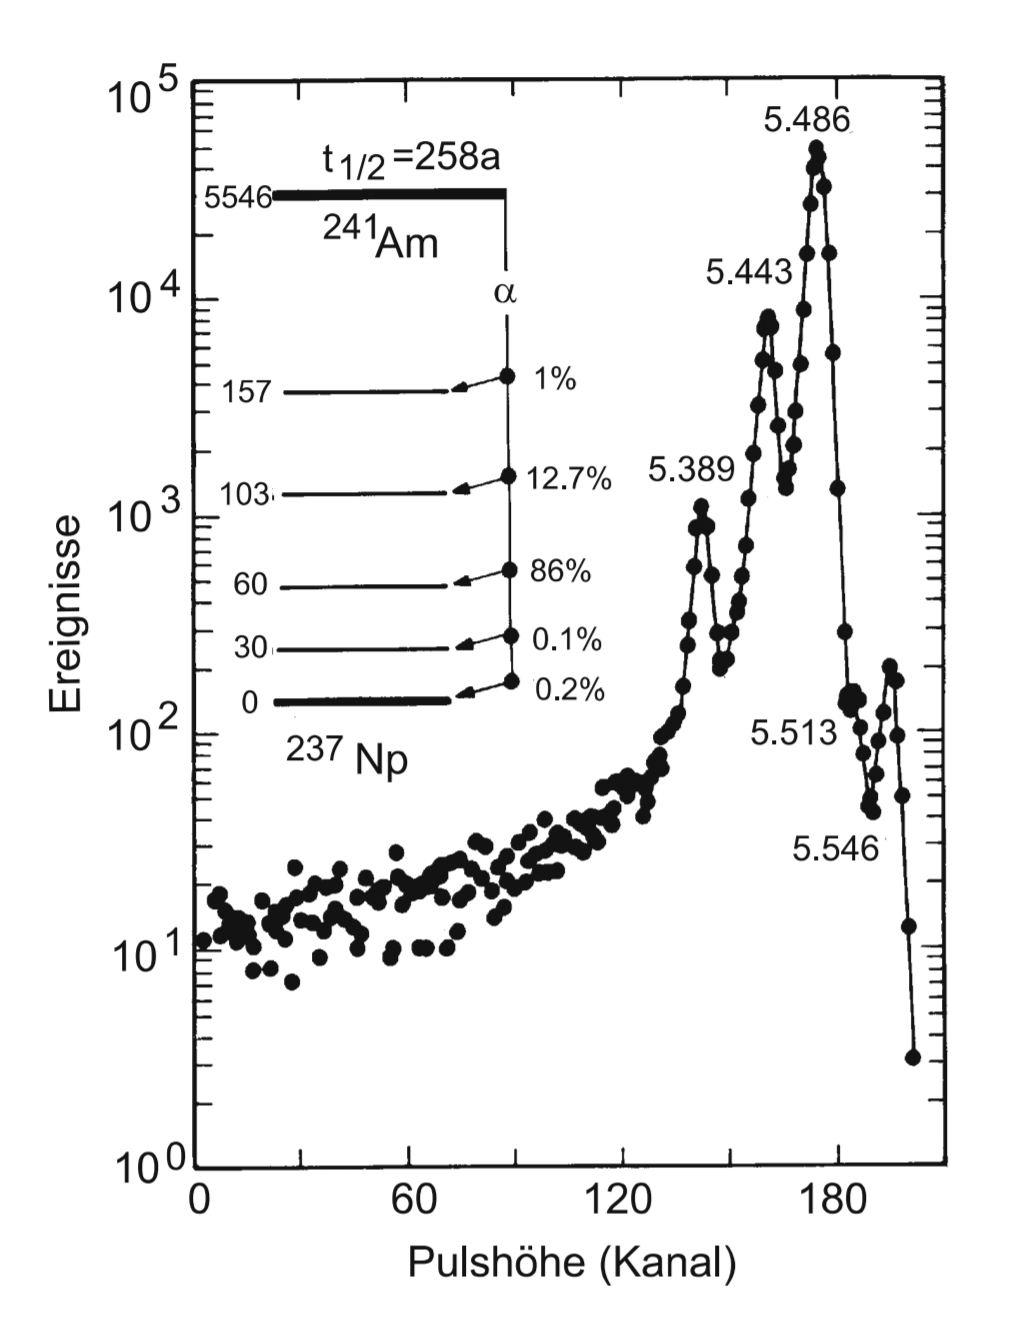
\includegraphics[width=\textwidth]{../media/B3.3/Am241_Spektrum.jpg}
		\caption{Energiespektrum von $\ce{^241Am}$, Quelle: \cite{Bethge}}
		\label{abb:Spektrum}
	\end{minipage}
	\begin{minipage}{0.45\textwidth}
		\centering
		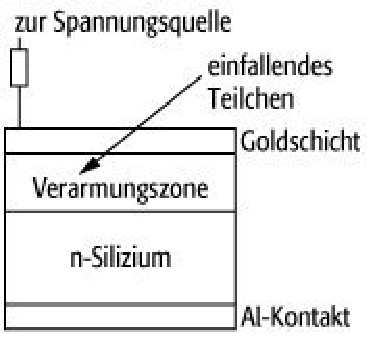
\includegraphics[width=0.7\textwidth]{../media/B3.3/Oberflaechensperrschichtzaehler.pdf}
		\caption{schematischer Aufbau eines Oberflächensperrschichtzählers,
			Quelle: \cite{Spektrum]}}
		\label{abb:Oberflächensperrschichtzähler}
		\vspace{1cm}
		
		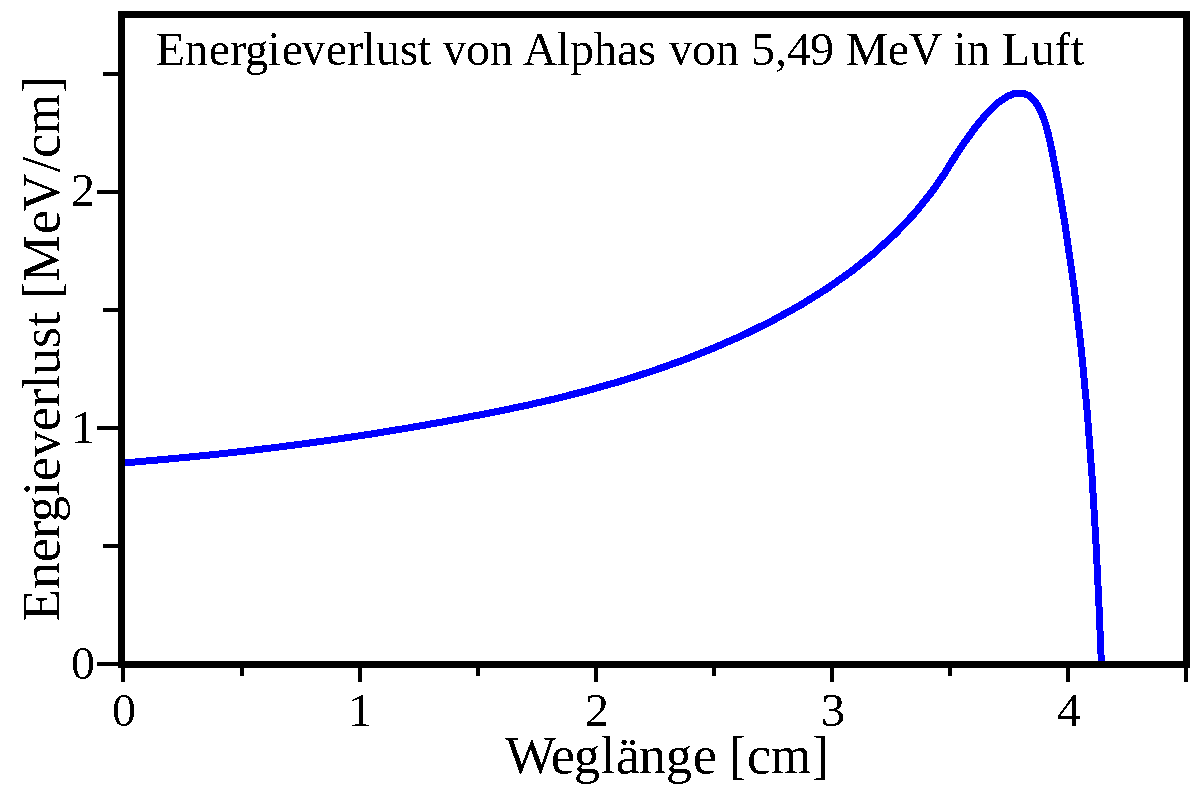
\includegraphics[width=\textwidth]{../media/B3.3/Bragg-Kurve.pdf}
		\caption{Bragg-Kurve von $\alpha$-Strahlung in Luft, Quelle: \cite{Alpha Luft}}
		\label{abb:Bragg-Kurve}
	\end{minipage}
	\vspace{1cm}
	
	\begin{minipage}{0.8\textwidth}
		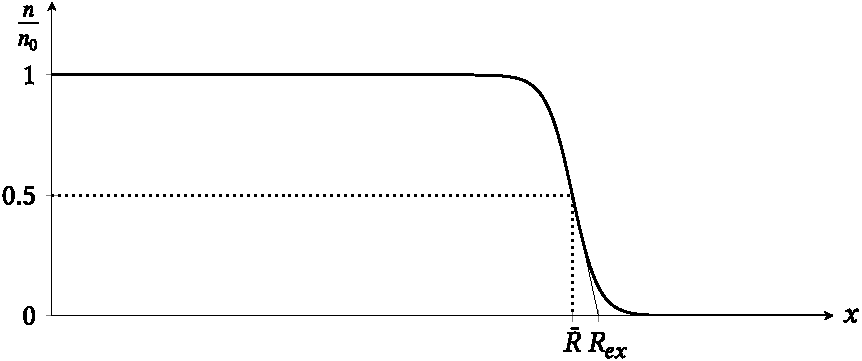
\includegraphics[width=\textwidth]{../media/B3.3/Reichweite.pdf}
		\caption{Intensität als Funktion der Eindringtiefe, Quelle: \cite{Uni}}
		\label{abb:Reichweite}
	\end{minipage}
\end{figure}

\clearpage

\begin{thebibliography}{99}
\bibitem{Bethge}
	K. Bethge, ``Kernphysik: Eine Einführung'', 3. Auflage,
	Springer-Verlag, 2008, ISBN: 9783540745679, DOI:
	\href{https://doi.org/10.1007/978-3-540-74567-9}{10.1007/978-3-540-74567-9}
\bibitem{Demtroeder}
	W. Demtröder, ``Experimentalphysik 4. Kern-, Teilchen und
	Astrophysik'', 3. Auflage, Springer-Verlag, 2010
\bibitem{Prior}
	Prior und Rollefson, ``Anomalous energy straggling of alpha
	particles'', American Journal of Physics, Mai 1982,
	\href{https://doi.org/10.1119/1.12834}{DOI 10.1119/1.12834}
\bibitem{CoN}
	``Chart of Nuclides'', National Nuclear Data Center,
	\url{https://www.nndc.bnl.gov/nudat3}, Abruf am 28.01.2024
\bibitem{Knoll}
	G. Knoll, ``Radiation Detection and Measurement'', Wiley, 2010, ISBN:
	9780470131480
\bibitem{Spektrum]}
	Lexikon der Physik, Spektrum Verlag,
	\url{https://www.spektrum.de/lexikon/physik/oberflaechensperrschichtzaehler/10568},
	29.01.2024
\bibitem{NIH}
	NIH National Library of Medicine NCBI, ``Ionization Energy in the
	Periodic Table of Elements'',
	\url{https://pubchem.ncbi.nlm.nih.gov/periodic-table/ionization-energy},
	Abruf am 28.01.2024
\bibitem{Uni}
	Universität zu Köln, ``Anleitung zum Versuch B3.3 - Reichweite von
	$\alpha$-Teilchen'', Januar 2021, Online verfügbar unter
	\url{https://www.ikp.uni-koeln.de/fileadmin/data/praktikum/B3.3_alpha_de.pdf},
	Abruf am 03.02.2024
\bibitem{Alpha Luft}
	Abbildung von $\alpha$-Strahlung in Luft: \url{https://commons.wikimedia.org/wiki/File:Bragg_Curve_for_Alphas_in_Air-PT-de.svg}, 2024-02-10
\bibitem{Bremsverm}
	Wikipedia, \url{https://de.wikipedia.org/wiki/Bremsvermögen}, 2024-02-10
\end{thebibliography}
\end{document}
